%%%%%%%%%%%%%%%%%%%%%%%%%%%%%%%%%%%%%%%%%%%%%%%%%%%%%%%%%%%%%%%%%%%%%%%%%%%%
% AGUJournalTemplate.tex: this template file is for articles formatted with LaTeX
%
% This file includes commands and instructions
% given in the order necessary to produce a final output that will
% satisfy AGU requirements, including customized APA reference formatting.
%
% You may copy this file and give it your
% article name, and enter your text.
%
%
% Step 1: Set the \documentclass
%
% There are two options for article format:
%
% PLEASE USE THE DRAFT OPTION TO SUBMIT YOUR PAPERS.
% The draft option produces double spaced output.
%

%% To submit your paper:
\documentclass[draft]{agujournal2019}
\usepackage{url} %this package should fix any errors with URLs in refs.
\usepackage{lineno}
\usepackage{color}
\graphicspath{ {figures/} }
\linenumbers
%%%%%%%
% As of 2018 we recommend use of the TrackChanges package to mark revisions.
% The trackchanges package adds five new LaTeX commands:
%
%  \note[editor]{The note}
%  \annote[editor]{Text to annotate}{The note}
%  \add[editor]{Text to add}
%  \remove[editor]{Text to remove}
%  \change[editor]{Text to remove}{Text to add}
%
% complete documentation is here: http://trackchanges.sourceforge.net/
%%%%%%%

\draftfalse

\journalname{JGR: Space Physics}


\begin{document}

\title{Statistical Properties of Electron Curtain Precipitation Derived with AeroCube-6}

%% ------------------------------------------------------------------------ %%
%
%  AUTHORS AND AFFILIATIONS
%
%% ------------------------------------------------------------------------ %%

\authors{M. Shumko\affil{1}, A.T. Johnson\affil{1},  T.P. O'Brien\affil{2}, D.L. Turner\affil{3}, J.G. Sample\affil{1}, J.B. Blake\affil{2}, L.W. Blum\affil{4}, A.J. Halford\affil{4}}


\affiliation{1}{Department of Physics, Montana State University, Bozeman, Montana, USA}
\affiliation{2}{Space Science Applications Laboratory, The Aerospace Corportation, El Segundo, California USA}
\affiliation{3}{Johns Hopkins Applied Physics Laboratory, Laurel, Maryland, USA}
\affiliation{4}{NASA's Goddard Space Flight Center, Greenbelt, Maryland, USA}


\correspondingauthor{M. Shumko}{msshumko@gmail.com}

\begin{keypoints}
\item We used the dual AeroCube-6 CubeSats to identify stationary, narrow, and persistent $>30$ keV precipitation in low Earth orbit
\item 90\% of curtains observed are narrower than 21 kilometers in latitude
\item A few curtains persistently scattered into the atmosphere for at least six seconds
\end{keypoints}


\begin{abstract}
Curtains are recently discovered stationary, persistent, and narrow in latitude electron precipitation phenomena observed in low Earth orbit over sequential passes of the dual AeroCube-6 CubeSats. The $> 30$ keV electron curtains were stationary over a variety of spacecraft separations, observed by the follower spacecraft up to 65 seconds after the leader. This study expands the recent curtain discovery and quantifies statistical properties of 1634 curtains observed over three years. We found that in low Earth orbit, many curtains are narrower than 10 kilometers in latitude and 90\% are less than 21 kilometers wide. We also found that curtains are an outer radiation belt phenomena that are observed in the late morning and midnight magnetic local time, with a higher occurrence rate at midnight. Furthermore curtains are observed more often at lower geomagnetic activity than microbursts.  We compare every statistical result to microbursts to test the hypothesis that curtains are drifting remnants of microbursts. Lastly, we found a few curtains in the bounce loss cone region in the north Atlantic Ocean where particle drift motion is impossible. In one such example, a curtain was continuously scattered for at least six seconds so curtains can be a significant source of $> 30$ keV electrons into the atmosphere.
\end{abstract}

\section{Plain Language Summary}

\section{Introduction}
Curtains are a stationary electron precipitation phenomena observed in low Earth orbit (LEO). They are narrow in latitude, spiky, and appear stationary for up to a minute between subsequent satellite passes. \citeA{Blake2016} recently discovered curtains with the $> 30$ keV electron dosimeters onboard the dual AeroCube-6 (AC6) CubeSats that operated together between 2014 and 2017. This discovery was possible due to AC6's actively maintained in-track separation between a few hundred meters and a few hundred kilometers. Besides the \citeA{Blake2016} discovery study not much is known about curtains including what they are, how are they generated, their statistical properties, and their impact on the atmosphere. Answering these questions is an essential next step towards a more complete understanding of how curtains, and particle precipitation in general, affect the magnetosphere and Earth.

Recently developed multi-spacecraft missions, such as AC6, are necessary to identify and distinguish curtains from similar-looking transient precipitation called electron microbursts. Microbursts have been observed since mid 1960s by high altitude balloons and satellites and are also a spiky increase of electrons shorter than a second but are not spatially stationary \cite<e.g.>{Anderson1964, Lorentzen2001a, O'Brien2003, Douma2017}. The  companion study to this work by \citeA{Shumko2020} calculated the spatial size of microbursts using simultaneous observations of microbursts observe by AC6. The impact of microbursts on the environment is substantial. \citeA{Lorentzen2001b}, \citeA{Thorne2005}, \citeA{Breneman2017}, and \citeA{Douma2019}---among others---estimated that microbursts can deplete the outer radiation belt electrons in about a day. Furthermore, \citeA{Seppala2018} modeled a 6 hour microburst storm and concluded that microbursts depleted mesospheric ozone by roughly 10\%. Thus, it is important to understand the connection, if any, between microbursts and curtains. Curtains and microbursts can be easily misidentified from a single spacecraft so we need to reevaluate single-satellite microburst studies. If curtains are numerous then the estimated microburst occurrence rates are overestimated. Furthermore, the microburst impact on the atmosphere and the outer radiation belt is overestimated.

\citeA{Blake2016} proposed the following hypothesis that explains curtain-microburst relationship. If a microburst is not completely lost in the atmosphere after the initial scatter, the remaining microburst electrons will spread out (bounce phase disperse) along the entire magnetic field line over a few bounce periods. Concurrently these electrons drift to the east, with higher energy electrons drifting at a faster rate. Therefore, the initially localized microburst is spread out in longitude into the shape of a curtain. \textcolor{red}{Maybe cite the curtain paper from 2000 that relates them to lightning? Title: Trapped energetic electron curtains produced by thunderstorm driven relativistic runaway electrons.}

The AC6 dosimeters lack the necessary pitch angle resolution to differentiate between drifting and precipitating electrons to test the \citeA{Blake2016} hypothesis. Instead we use AC6's position and Earth's asymmetric magnetic field to differentiate particles that are either nearly-trapped in the drift loss cone, and particles immediately lost in the bounce loss cone (BLC). These concepts are described below.

Earth's magnetic field is spatially shifted towards Singapore which creates a region of weaker magnetic field in the South Atlantic Ocean called the South Atlantic Anomaly (SAA). This magnetic field asymmetry allows particles to mirror much closer to Earth's surface and possibly be lost in the SAA. Most particles observed in LEO are barely-trapped: they bounce and drift around the Earth until they reach the SAA. Here the weaker magnetic field strength lowers the electron's mirror point into the atmosphere where collisions with the atmosphere are more numerous and the particle is lost. Particles that drift and are lost in the SAA have pitch angles in the drift loss cone. Particles with smaller pitch angles that are unable to complete a full bounce, and are immediately lost in the atmosphere, are in the BLC. Traditionally, a particle in the BLC mirrors at or below an altitude of 100 kilometers. In this study we will use this definition of the BLC as well as a more strict definition of a mirror point below sea level.

Without pitch angle resolution AC6 can not easily differentiate between trapped, drift loss cone, and bounce loss cones electrons. In the SAA, AC6 observes a combination of trapped, drift loss cone, and BLC electrons. In most regions, outside of the SAA and its conjugate point, AC6 will observe electrons in the drift and bounce loss cones. Lastly, when AC6 is in the region conjugate to the SAA in the North Atlantic, it only observes particles in the BLC. A particle is in the BLC if its conjugate mirror point is below 100 km. If an electron makes it to AC6's altitude, it can be in the local loss cone and precipitate in the local hemisphere. Alternatively, the electron will mirror at or below AC6 and gyrate into the SAA where the equivalent mirror point magnetic field strength is deep in the atmosphere or below sea level. Therefore, any precipitation observed in the BLC region in the North Atlantic must rapidly precipitate.

\textcolor{red}{Think about how Max Comess explained the BLC. Am I going overboard?... ``The bounce loss region is defined as
where the field of view of the PET and HILT detectors are
fully within the bounce loss cone, where the bounce loss cone
is defined such that any electrons detected should precipitate
on their next bounce, ensuring that any particles viewed by
SAMPEX in this region are not trapped, nor were they
scattered into the loss cone at a substantially different MLT
than SAMPEX’s location. These criteria put SAMPEX in
the north Atlantic (Figure 1), conjugate to the outer-belt
portion of the South Atlantic Anomaly [see, e.g., Dietrich
et al., 2010, Figure 3]."}

This study expands the \citeA{Blake2016} study by estimating statistical properties of curtains and address the \citeA{Blake2016} hypothesis. We use 1634 confirmed curtain observations to learn about the distributions of: the curtain width in latitude, the geomagnetic conditions favorable to curtains, and curtain distribution in L and magnetic local time (MLT). Lastly we will address the hypothesis that curtains are drifting remnants of microbursts by showing examples of curtains observed in the BLC region.

\section{Instrumentation} \label{instrumentation}
The AC6 mission was a pair of 0.5U (10x10x5 cm) CubeSats built by The Aerospace Corporation designed to measure the electron and proton environment in low Earth orbit \cite{O'brien2016}. AC6 was launched on 19 June 2014 into a 620x700 km, $98^\circ$ inclination orbit. The AC6 orbit over the three year mission lifetime was roughly dawn-dusk, and precessed only a few hours in MLT; 8-12 MLT in dawn and 20-24 MLT in dusk. The two AC6 spacecraft, designated as AC6-A and AC6-B, separated after launch and were in proximity for the duration of the three year mission---maintained by an active attitude control system. The attitude control system allowed them to precisely control the amount of atmospheric drag experienced by each AC6 unit using the surface area of their solar panel ``wings". By changing their orientation, AC6 was able to maintain a separation between 2-800 km, confirmed with the Global Positioning System. The two AC6 units were in a string of pearls configuration so one unit, typically unit A, was leading the other by an in-track lag---the time it would take the following spacecraft to catch up to the position of the leading spacecraft. To convert between the AC6 in-track separation and in-track lag, we assume a typical 7.5 km/s orbital velocity of LEO spacecraft. The in-track lag was readily available with the Global Positioning System which makes it easy to study precipitation phenomena observed at the same time, and at the same position by shifting one time series by the in-track lag.

Each AC6 unit contains three Aerospace microdosimeters (licensed to Teledyne Microelectronics, Inc) that measure the electron and proton dose in orbit \cite{O'brien2016}. The dosimeter used for this study is dos1 with a $30$ keV electron threshold. dos1 is used for this study because the other dosimeters either responded primarily to protons or were not identical between unit A and B. All dosimeters sample at 1 Hz in survey mode, and 10 Hz in burst mode. 10 Hz data was readily available from both AC6 units from June 2014 to May 2017 while their in-track lag was less than 65 seconds, and at times was a fraction of a second. \textcolor{red}{Show a distribution of the in-track lag when they had 10 Hz data?} The variety of AC6 separations and data availability over the three-year mission makes it possible to study tranisent electron microburst precipitation \cite{Shumko2020} and now stationary electron curtain precipitation.

\section{Methodology} 
\subsection{Curtain Identification} \label{curtain_identification}
The 10 Hz data was used to identify curtains with the following two criteria: a high spatial correlation, and spiky. The first criterion quantifies the similarity of the feature between both AC6 units, and the second criterion checks that highly correlated times were spiky. Before we applied the identification criteria, the AC6-B time series was shifted by the in-track lag to spatially align it with the AC6-A time series. 

The first identification criterion is a 1-second rolling Pearson correlation applied to both time series. Spatial features with a correlation greater than 0.8 are considered highly correlated.

The second identification criterion, applied to the highly correlated locations identified by the first criterion, identifies locations where both AC6 units observed spiky precipitation. Similar to how precipitation bands were identified by \citeA{Blum2015} and microbursts by \citeA{Greeley2019}, we find spiky precipitation by quantifying the number of Poisson standard deviations, $\sigma$, that a dos1 count rate is above a 10-second centered running average, $B_{10}$. Locations where dos1 is at least two $\sigma$ above $B_{10}$, in other words $dos1 > 2\sqrt{B_{10}} + B_{10}$, are spiky. 

The locations where the two criteria are met are curtain candidates and the time of the peak count rates are saved. We tuned the detection parameters to have as many candidate curtains as possible while being feasible to inspect every detection. To check the quality of the data set, one author visually checked every candidate curtain and 1634 curtains were confirmed. Four curtain examples are shown in Fig. \ref{fig1}. In each example, the unmodified time series is shown in the top row and the spatially-aligned time series the bottom row. The in-track lag used to shift the bottom row is annotated by $dt$, corresponding to an AC6 in-track separation annotated by $s$. The top row is uncorrelated so these events were not microbursts. The bottom row is correlated at the same location after 3 to 26 seconds. The correlated curtains in the bottom row are peculiar---their fine width is on a 10-kilometer scale and was observed to persist for at least 26 seconds.

\begin{figure}
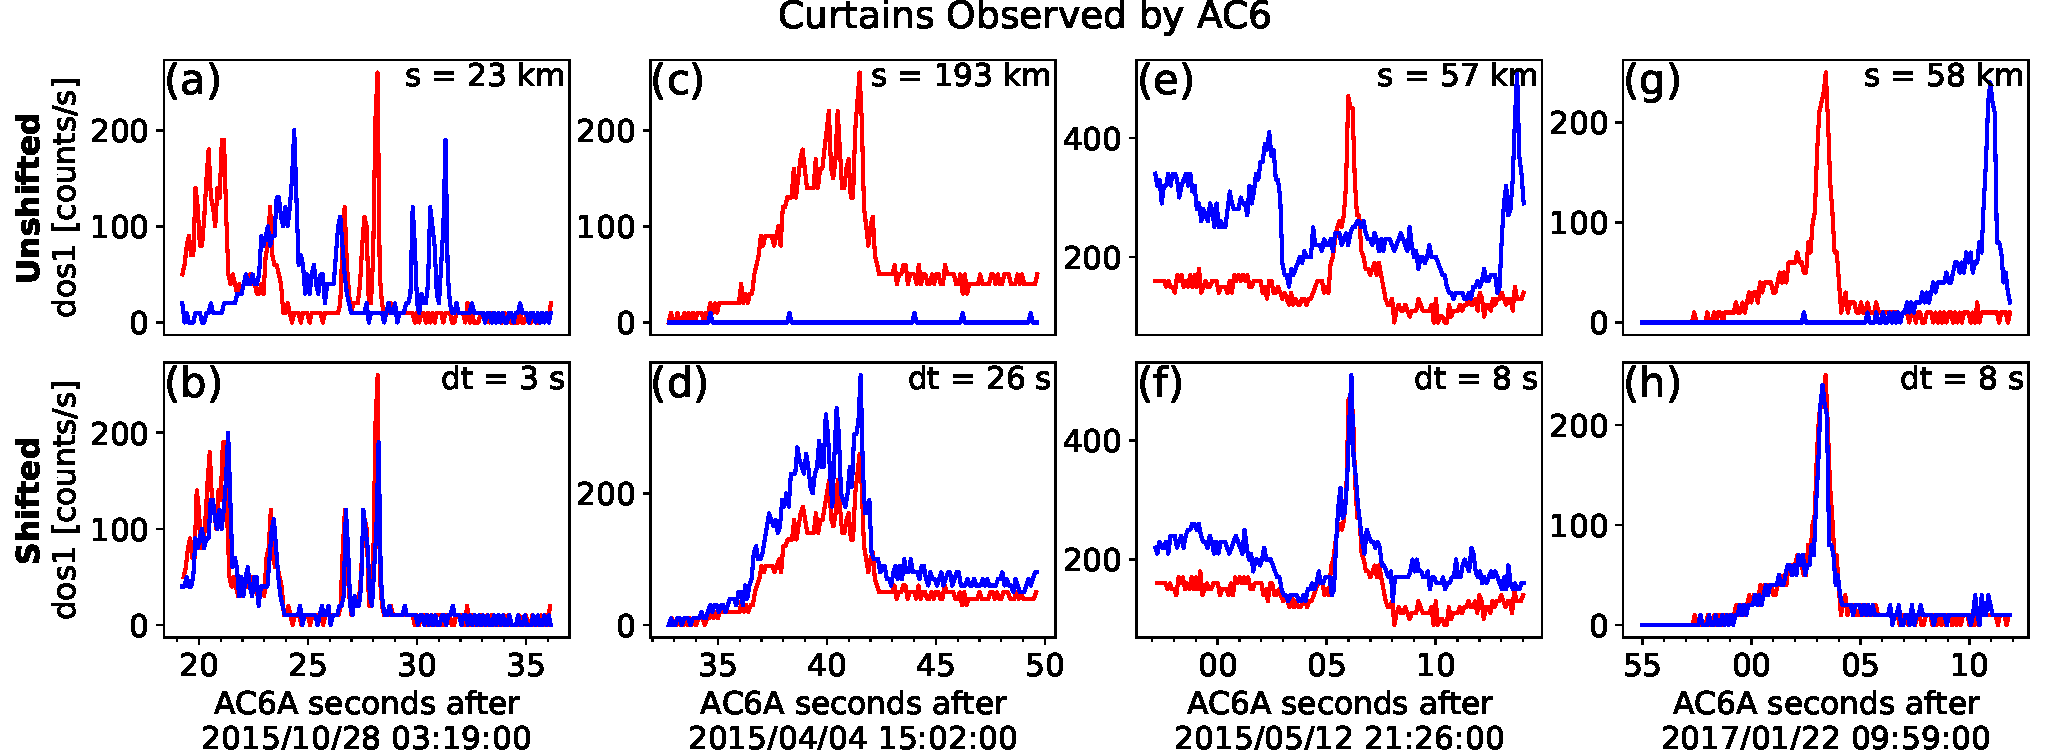
\includegraphics[width=\textwidth]{fig1.pdf}
\caption{Four examples showing the AC6 $> 30$ keV electron data taken by AC6 at the same time in the top row and at the same position in the bottom row. AC6-A, whose data is shown with red curves, was $s$ kilometers ahead of AC6-B. To show the data at the same position the time series data from one spacecraft was shifted by the in-track lag and annotated by dt. These examples show that curtain precipitation was highly correlated for up to 26 seconds.}
\label{fig1}
\end{figure}

\section{Results} \label{results}
In the spirit of brevity, we limited the scope of this statistical study to answer three questions:

\begin{enumerate}
\item How narrow are curtains?
\item When and where are curtains observed?
\item Are curtains drifting or locally precipitating?
\end{enumerate} For each of these questions we will compare the curtain distribution with the $>30$ keV microburst distribution from \citeA{Shumko2020}. Lastly, we will show evidence that suggests that some curtains are continuously scattered and not drifting.

\subsection{Curtain Width}
We quantified curtain width in time as the width at half of the curtain's topographic prominence: the height of the peak above the lowest contour that encircles the peak but contains no higher peak. The spatial width of a curtain is the product of the temporal width and the 7.5 km/s orbital velocity mostly in latitude. The distribution of curtain widths is shown in Fig. \ref{width_dist} by the thick black curve. Curtains are very narrow in latitude. Many curtains are less than 10 km wide, and 90\% are narrower than 21 km.
	
We compared the curtain width distribution to the microburst size distribution estimated in \citeA{Shumko2020}. \citeA{Shumko2020} estimated the microburst size distribution by finding microbursts that were observed simultaneously by both AC6 units so the microburst size much be larger than the AC6 separation. The red curve in Fig. \ref{width_dist} shows the microburst distribution estimated from the ratio of the number of concurrent and nonconcurrent microbursts observed in each separation bin. 

The curtain and microburst size distributions are very similar with a one notable difference. Curtain widths are observed directly hence their distribution is peaked, while the microburst distribution is estimated from concurrent observations so their distribution is peaked at 0 km AC6 separation. \textcolor{red}{something something ... as one would expect if curtains measure the entire region of instability, whereas individual microbursts only represent sub-regions within that which become unstable at different times.}

\subsection{When and Where Are Curtains Observed}
The distribution of curtains in L and MLT is shown in Fig. \ref{l_mlt_dist}. Figure \ref{l_mlt_dist}a shows the distribution of the 1634 observed curtains and Fig. \ref{l_mlt_dist}b shows the normalized distribution. The white bins, mostly in the early morning and evening MLT regions, had no observed curtains because the AC6 orbit did not sample there. Figure \ref{l_mlt_dist}c confirms this by showing the distribution of the number of quality (data quality flag = 0) 10 Hz samples.

After scaling by the uneven sampling in the late morning and midnight MLT regions, the normalized distribution in Fig. \ref{l_mlt_dist}b shows enhanced curtain occurrence in the outer radiation belt in late morning and midnight MLT regions.

Now we quantify the geomagnetic conditions favorable for curtains. Figure \ref{ae_dist} shows the distribution of the Auroral Electroject (AE) index between 2014 and 2017, and the distribution of the AE index when curtains and microbursts were observed. The distribution of the AE index when $> 30$ keV microbursts were observed is shown with a dashed green curve. Curtains are observed typically when AE is enhanced. Microbursts are observed when AE is enhanced more than for curtains.

\begin{figure}
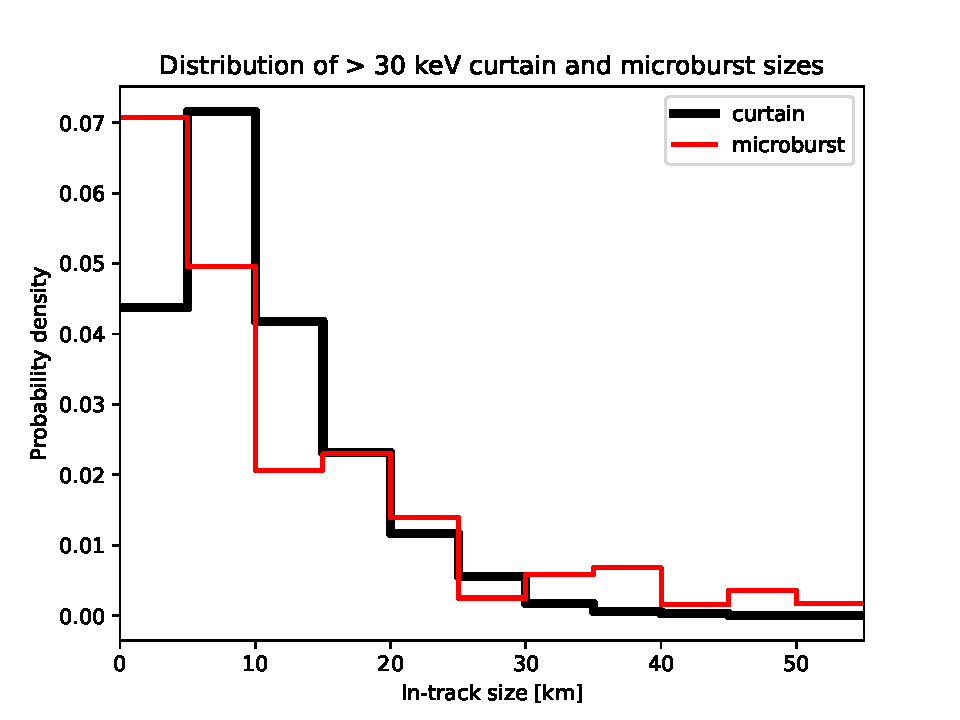
\includegraphics[width=\textwidth]{ac6_curtain_microburst_width_dist.pdf}
\caption{Distribution of curtain width in latitude shown in black and sizes of microbursts when they were simultaneously observed by AC6 is shown in red. Microburst distribution adopted from \citeA{Shumko2020}. The error bars represent the Poisson standard error.}
\label{width_dist}
\end{figure}

\begin{figure}
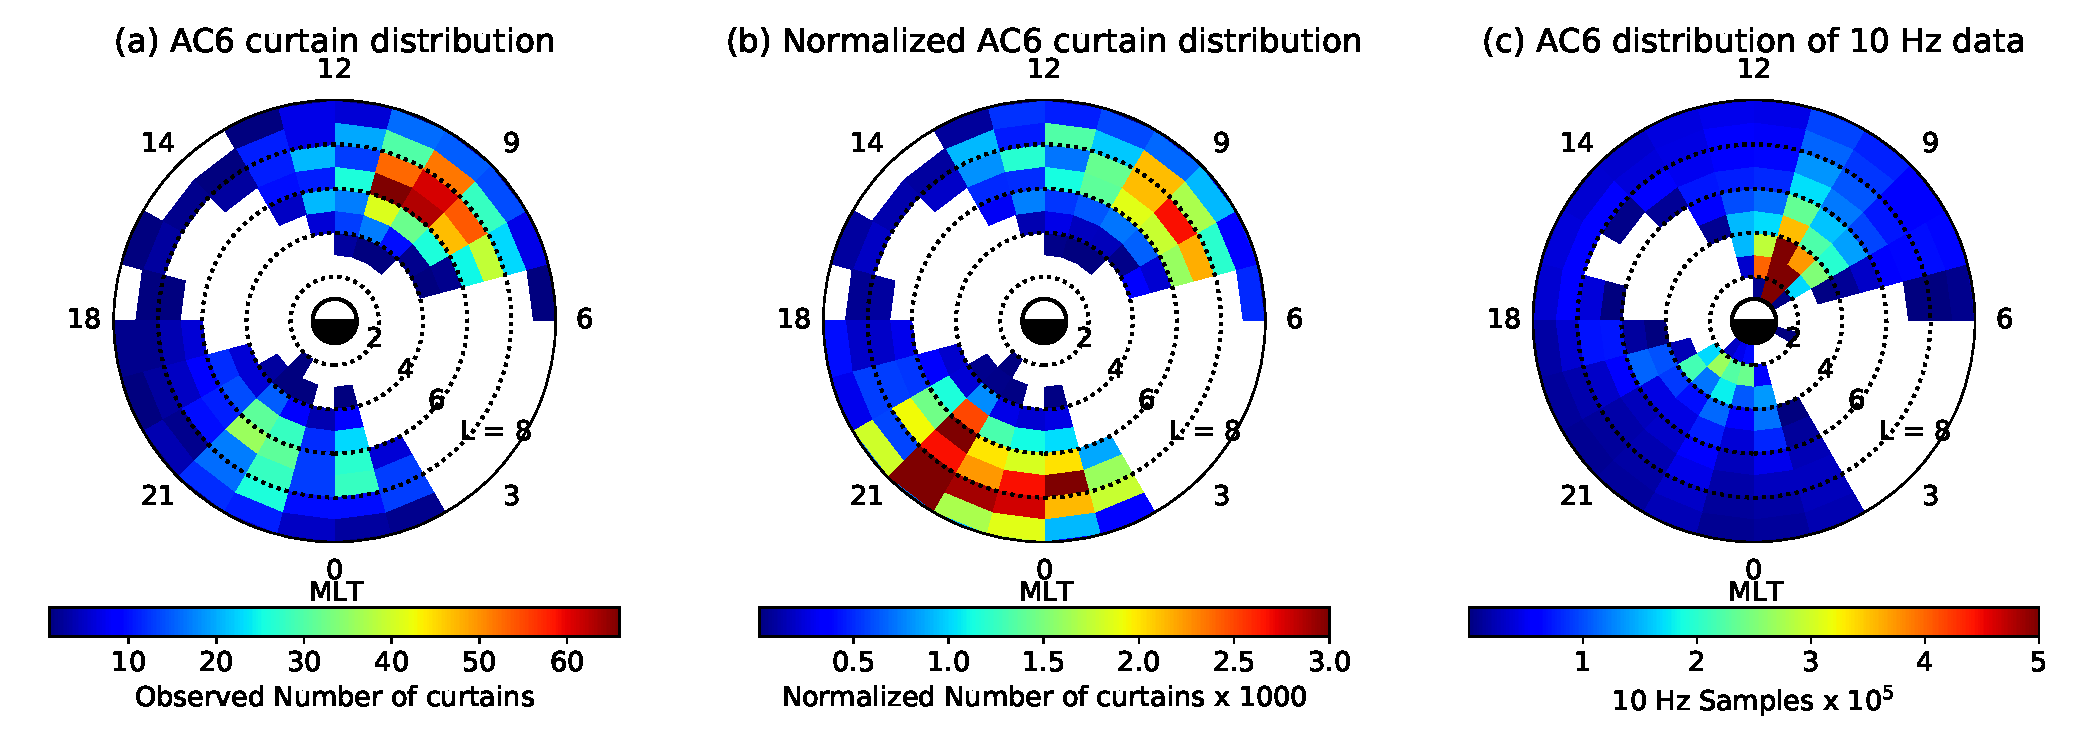
\includegraphics[width=\textwidth]{fig2_2.pdf}
\caption{Distribution of observed curtains as a function of L and MLT in panel a and normalized number of curtains in panel b. Panel c shows the number of quality 10 Hz samples taken at the same time that was used to normalize panel b. The white bins in panels a have 0 curtain observations. In panel b the white shaded bins had either 0 detections or very little 10 Hz samples (less than $10,000$).}
\label{l_mlt_dist}
\end{figure}

\begin{figure}
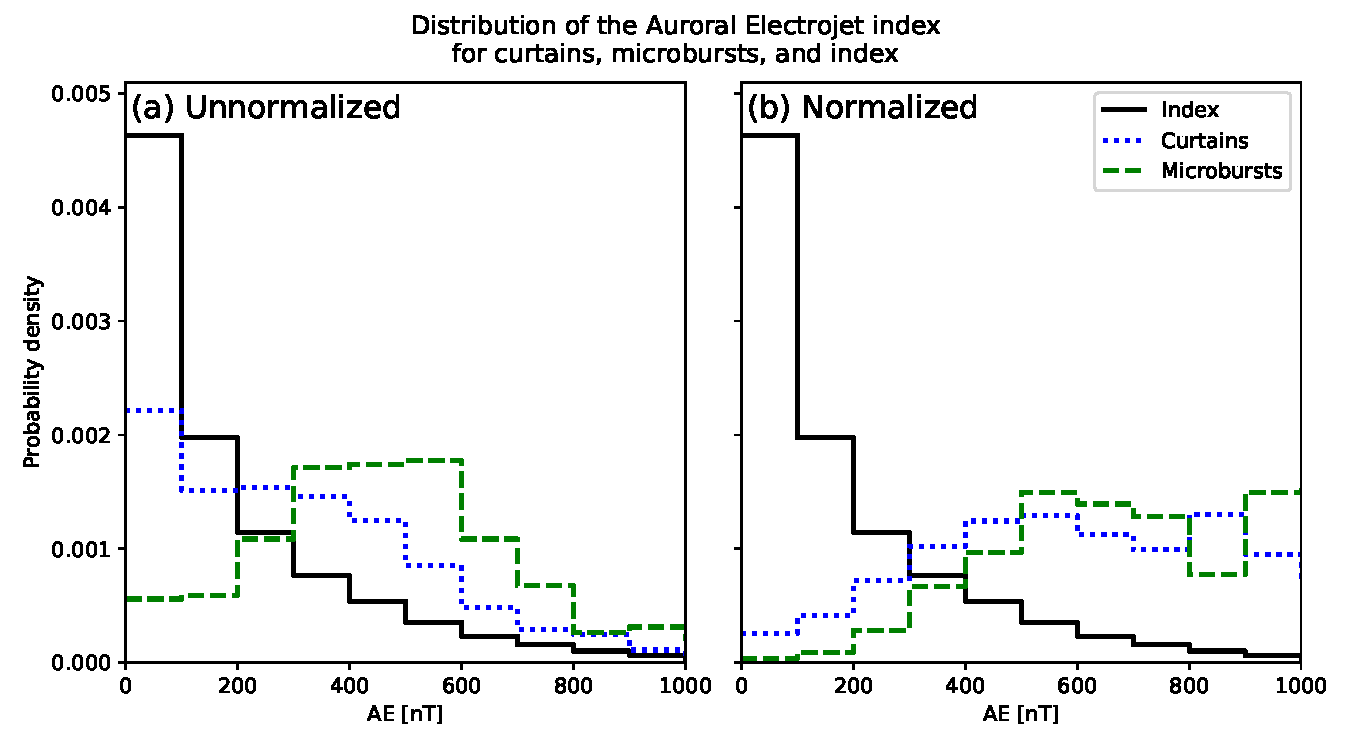
\includegraphics[width=\textwidth]{ac6_curtain_microburst_AE_dist.pdf}
\caption{The distribution of the Auroral Electroject (AE) index from 2014 to 2017. The black curve shows the distribution for the entire 2014-2017 AE data set, the dotted blue curve shows the AE distribution for curtains, and the dashed green curve shows AE the distribution for microbursts studied in \citeA{Shumko2020}.}
\label{ae_dist}
\end{figure}

\subsection{Local Atmospheric Precipitation}
\textcolor{red}{The evidence presented so far hint at, but not directly confirm that, curtains are connected to microbursts. But there are a few curtain observations that put the hypothesis into question. }
Now we will show examples of curtains that were scattered over an extended period of time in the BLC. We estimated the BLC region in the North Atlantic Ocean using the IRBEM-Lib magnetic field library \cite{irbem}. First we estimated the local magnetic field strength on a latitude-longitude grid spanning the North Atlantic, at 700 kilometer altitude that is typical for AC6. For each latitude-longitude point we traced that magnetic field line to the SAA and found the position along that field line with an equivalent field strength as in the North Atlantic. A particle that mirrors at the grid location will mirror and gyrate to the southern hemisphere before mirroring at an altitude with the equivalent field strength or be lost in the atmosphere. Since we are considering particles mirroring at the grid points in North Atlantic, this estimate is the upper bound altitude that the particle can mirror. Particles mirroring above the grid will not be observed, and the particles that are observed will mirror at or below the estimated altitude in the SAA. If the corresponding field strength position is at 100 kilometers or lower in the SAA we considered that grid point in the North Atlantic in the BLC region. For the more rigorous BLC criteria, we saved the grid locations where the equivalent field strength altitude in the SAA is below sea level. 

Figure \ref{fig3}a shows a map of the BLC region in the North Atlantic. The solid blue line is the north bound of the region where a particle observed at 700 kilometers at that location will mirror at 100 kilometers in the SAA. Immediately south of the solid blue line the SAA mirror altitude rapidly decreases towards, and below, sea level. The dashed blue line is the set of latitude-longitude points where the SAA mirror point altitude is at sea level. Furthermore we superposed two dotted black lines on Fig. \ref{fig3}a that represent the boundary of the outer radiation belt defined between L shells of 4 and 8. The BLC region here closely matches the region shown in \citeA[Figure 1]{Comess2013} and \citeA[Figure 3]{Dietrich2010}. We used the Olson-Pfitzer magnetic field model \cite{Olson1982} to estimate the BLC boundary. The same analysis using the Tsyganenko 1989 model \cite{Tsyganenko1989} yielded similar boundaries. 

We found four good curtains that were observed inside the BLC regions and included the shifted time series plots in Fig. \ref{fig3}b-e, with the AC6 in-track lag, L and MLT of the observations annotated. The AC6 locations where these curtains were observed are shown in \ref{fig3}a with red stars and the corresponding panel labels. The curtains shown in Fig. \ref{fig3}c and e were observed near the sea level SAA mirror altitude curve thus they were not drifting and were precipitating as much as 6 seconds as shown in Fig. \ref{fig3}e. For reference, the precipitation persisted for longer than the typical $\approx 1.5$ second bounce period of 30 keV electrons in this region.

\textcolor{red}{These examples were observed near the sea level BLC curve, so at a minimum, those electrons would have gyrated down to sea level in the South Atlantic Anomaly. This is a very conservative estimate because the observed electrons likely mirrored below AC6 and thus below sea level (if Earth was not in the way). Figure 3 casts doubt on the microburst-curtain hypothesis but more work will be necessary to fully conclude if microbursts and curtains are related. These examples were observed near the sea level BLC curve, so at a minimum, those electrons would have gyrated down to sea level in the South Atlantic Anomaly. This is a very conservative estimate because the observed electrons likely mirrored below AC6 and thus below sea level (if Earth was not in the way). Figure 3 casts doubt on the microburst-curtain hypothesis but more work will be necessary to fully conclude if microbursts and curtains are related. }

\begin{figure}
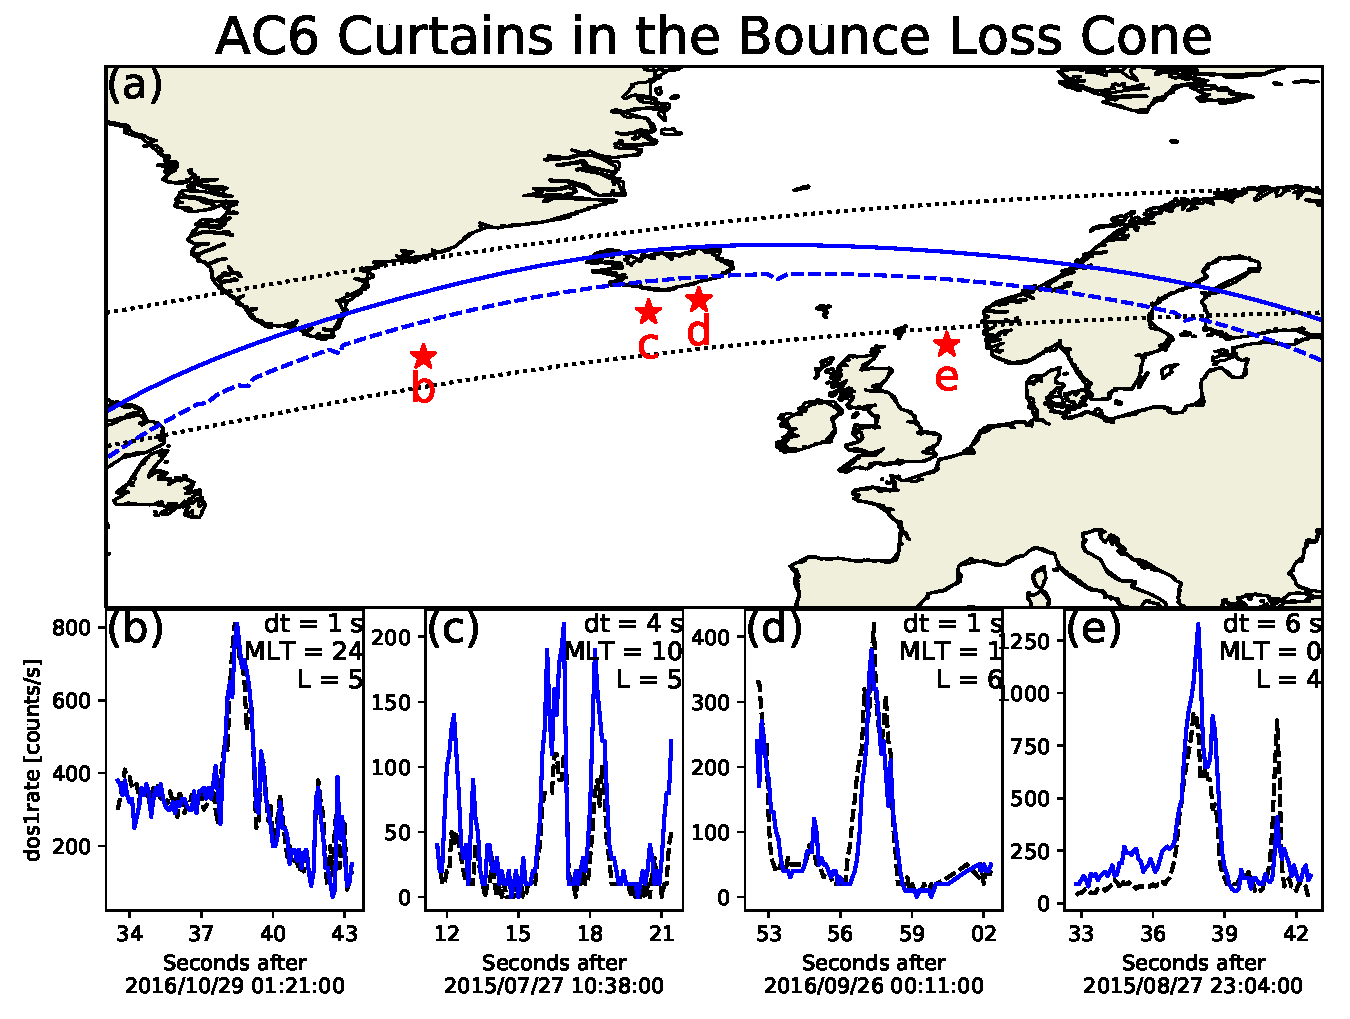
\includegraphics[width=\textwidth]{fig3.pdf}
\caption{Curtains observed inside the bounce loss cone region. Panel a shows a map of the North Atlantic region with the outer radiation belt, defined by an L shell range between 4 and 8, shown with the dotted black curves. The solid blue curve shows the northern boundary of the bounce loss cone region. Along this curve, electrons observed at a 700 kilometer altitude in the North Atlantic will mirror at 100 kilometers in the SAA. A more strict bounce loss cone criteria is the dashed blue curve that represents a mirror point altitude at sea level in the SAA. The 4 red stars with labels show the locations of the curtain examples shown in panels b-e. The panels b-e show the 4 example curtains with the AC6-A shown by the red line, and AC6-B with the blue line. AC6-A was ahead in all examples except panel d.}
\label{fig3}
\end{figure}

\section{Discussion} \label{discussion}
\subsection{Curtain Width In Latitude}
Curtains are very narrow in latitude. Figure \ref{width_dist} shows the width in latitude of many curtains are on the order of 10 kilometers and 90\% are narrower than 21 km. Scaled to the magnetic equator, where we presume curtains are generated, these latitudinal widths correspond to a source with a radial scale size of a few hundred kilometers. As shown in Fig. \ref{fig1}f and \ref{fig1}h; it is remarkable that some curtains maintain a fine structure after multiple seconds with little observable difference. Sometimes curtains appear to be slightly and systematically shifted in latitude, while maintaining their shape (not shown).

If curtains are remnants of microbursts then the distribution of curtain widths in latitude correspond to the microburst size distribution. Figure \ref{width_dist} shows a good correspondence between the distribution of curtain widths in latitude and the microburst size distribution from \citeA{Shumko2020}. Therefore, it is reasonable to believe that curtains and microbursts are related, but this result need to be closely inspected for sources of bias. 

The microburst scale size distribution, as described in \citeA{Shumko2020}, is the fraction of microbursts observed simultaneously to all microbursts observed either simultaneously or by only one AC6 unit. A microburst observed simultaneously must be larger than the spacecraft separation so the microburst distribution represents a lower bound. \citeA{Shumko2020} attempted to account for this bias but it is difficult. This bias that shifts the microburst distribution to smaller sizes so in the microburst size distribution shown in Fig. \ref{width_dist} is underestimated.

Furthermore the detection algorithm described in section \ref{curtain_identification} has a width bias. For wide curtains with a similar width to the detection algorithm's 10-second baseline, the 10-second baseline is then calculated using the enhanced curtain counts instead of the background and is increased above the true background and thus the curtain peak is less pronounced relative to the baseline. As a result, the curtain detection algorithm is less sensitive to wider curtains. The result of this bias is similar to the bias inherent in the microburst distribution---the curtain widths are underestimated.

Both of these biases underestimate the true size of curtains and microbursts, so this evidence agrees with the \citeA{Blake2016} microburst-curtain hypothesis.

\subsection{When and Where Are Curtains Observed}
Figure \ref{l_mlt_dist} shows that curtain phenomena originates in the outer radiation belt, and observed relatively more in the evening than morning regions. Unfortunately, the limited AC6 coverage prevents a complete curtain distribution in MLT. From the MLT information we have in Fig. \ref{l_mlt_dist}b, curtains are most often observed near midnight MLT with relatively less observed in the late morning MLT. This distribution, though limited, appears to be similar to the L-MLT distribution of microbursts from prior studies \cite<e.g.>{O'Brien2003, Douma2017}.

Curtains also exhibit a preference to disturbed geomagnetic conditions as shown in Fig. \ref{ae_dist}, but not as disturbed as microbursts from \citeA{Shumko2020}. A possible explanation: during quiet conditions the remnant microburst electrons are more likely to drift undisturbed and AC6 is more likely to observe the fine, highly-correlated curtain structure. In contrast, during active conditions curtain electrons are still drifting, but the dynamics of an actively-changing magnetosphere can easily perturb curtain electrons until AC6 no longer observes a highly correlated structure at the same location.
 
\subsection{Curtains Observed in The Bounce Loss Cone}
Lastly we address curtains observed in the bounce loss cone. What can cause continuous $>30$ keV electron precipitation lasting for multiple seconds? This mechanism must be radially localized near the magnetic equator, on a scale of a few hundred kilometers. A candidate mechanism is a direct current electric field that is parallel to the background magnetic field that lowers the electron mirror point to AC6 altitudes. To find the minimum potential we assume the electron is barely trapped and has a mirror point at 100 kilometers in the SAA (and will likewise mirror above AC6's altitude in the conjugate point). This condition implies that the particle's mirror point in the bounce loss cone is above AC6. 

To find the parallel potential potential we use the kinetic energy, $W$, of a $30$ keV particle at its initial mirror point at a magnetic field strength of $B_i$. The kinetic energy at the initial mirror point can be written as $W_i = \mu B_i$ where $\mu$ is the first adiabatic invariant. Now when a parallel potential acts on the electron of charge $q$ and does $q \Phi$ amount of work, the electron will mirror closer to Earth's surface and mirror at a field strength $B_f$ where its final energy is $W_f = \mu B_f$. \textcolor{red}{In this derivation we assume that the work done on the electron is a small fraction of its kinetic energy.} Now we relate the initial and final kinetic energy of the electron,

\begin{equation}
\mu_f B_f = \mu_i B_i + q \Phi
\end{equation} which after we rearrange, and substitute $\mu$ assuming it does not change, the above expression is approximately

\begin{equation}
 q \Phi \approx W \frac{(B_f - B_i)}{B_i}.
\end{equation}

We again use IRBEM-Lib to estimate $ q \Phi$. For each example curtain in Fig. \ref{fig3}, we first estimated the local magnetic field, $B_f$ for this derivation. Then we traced the field line from AC6 into the SAA. We found $B_i$ at 100 kilometers altitude in the SAA for barely trapped electrons. With the initial and final $B$, along with $W = 30$ keV, the minimum potential must be $q \Phi = 1-4$ kV. \textcolor{red}{Recalculate the potentials for the four cases.}. This range of potentials is typical for the aurora. \citeA{Partamies2008} used the observations made by the Fast Auroral SnapshoT (FAST) mission and reported that the inverted-V auroral structures, observed up to a few tens of keV, were accelerated by 2-4 kV potentials. While the aurora and curtains are likely different, the aurora is observed at higher L and near midnight MLT region, they do share a number of similarities. If AC6 had differential energy channels below 30 keV, then it would be possible to test a possible relationship between curtains and inverted-V structures.

Outside of the BLC, the lack of pitch angle information makes the AC6 electron data ambiguous, but the curtains observed in the BLC suggest that some curtains continuously precipitate for multiple seconds. Curtains could be a significant source of energetic particles into the atmosphere. Energetic electron precipitation generates odd Nitrogen ($\mathrm{HO_X}$) that is currently underestimated by atmospheric models such as the widely-used Whole Atmosphere Community Climate Model using Specified Dynamics (SD-WACCM) \cite<e.g.>{Randall2015}. A comprehensive study of the curtain impact on the atmosphere should be done with an AC6-like mission with pitch angle and energy resolution. 


\section{Conclusions}
The 1634 confirmed curtains allowed us to make the following statistical inferences:

\begin{enumerate}
\item Curtains are very narrow---90\% are less than 21 kilometers wide in latitude.
\item Curtains are observed in the outer radiation belt, predominately in the midnight and the late morning MLT regions, during periods of moderate geomagnetic activity.
\item Some curtains continuously precipitate into the atmosphere for multiple seconds.
\end{enumerate}

Curtains are remarkably narrow with fine structure that persist for multiple seconds. Either the scattering mechanism that contentiously generates curtains is physically static for multiple seconds, or the curtain electron drift is often undisturbed. 

The curtain-microburst relationship hypothesized in \citeA{Blake2016} is not clear. The two results in support of the hypothesis are: curtain width and microburst size distributions are very similar, and the limited AC6 sampling in MLT shows that both occur in similar locations in the magnetosphere. But the bounce loss cone result complicates this interpretation. Some curtains continuously precipitate for at least a few seconds and can be a significant source of energetic electron precipitation into the atmosphere. Furthermore, the continuous scatter of curtain electrons can be explained by a parallel direct current electric field and could be related to the aurora.

% \appendix

\acknowledgments
This work was made possible with the help from the many engineers and scientists at The Aerospace Corporation who designed, built, and operated AC6. M. Shumko was supported by NASA Headquarters under the NASA Earth and Space Science Fellowship Program - Grant 80NSSC18K1204. D.L. Turner is thankful for support from the Van Allen Probes mission and a NASA grant (Prime award number: 80NSSC19K0280). The work at The Aerospace Corporation was supported in part by RBSP-ECT funding provided by JHU/APL contract 967399 under NASA's Prime contract NAS501072. The AC6 data is available at http://rbspgway.jhuapl.edu/ac6 and the IRBEM-Lib version used for this analysis can be downloaded from https://sourceforge.net/p/irbem/code/616/tree/.

\section{Homeless Words}

Title: Statistical Properties of Curtains--Latitudinally-Narrow and Persistent Electron Precipitation Phenomena

This study leverages AC6, a multi-spacecraft mission, to interpret and understand particle precipitation in a way that is impossible with a single spacecraft.

This study leverages the asymmetry in Earth's magnetic field. The asymmetric magnetic field results in the SAA and the BLC, two very related and unique regions

Particles that impact the atmosphere are lost during that bounce motion. We found curtains in the bounce loss cone, a region in the North Atlantic near and above Iceland.

The bounce loss cone is magnetically connected to the SAA, where Earth's magnetic field is weakest near Earth's surface. A particle observed in the blc in the northern hemisphere will descend below 100 km altitude. At sub-100 km altitudes the particle has a high chance of encountering and scattering with the atmosphere and be lost. 

We found curtain electrons that, when given the chance to execute their cyclical bounce motion, will descend below Earth's surface in the SAA. An electrons can not survive that trip.

Write the paper and ask the question: "What is this paper really about?" Not just curtains, but uncovering something unexpected that has been observed and overlooked for decades.

Are curtains related to aurora? This is a good question---one that is not pertinent here (idea from The Elements of Style p.68).

Here are two parting questions that are not considered here. Why were some curtains shifted slightly? Perhaps it was due to the movement of the magnetic field lines. Also do curtains have a corresponding visual signature on the ground? The answer to this question will show if curtains are related to the aurora.

\bibliography{/home/mike/Dropbox/0_firebird_research/A_presentations/refs}
%\bibliography{"refs"}

\end{document}